\newcommand{\nom}{Porte conteneur}
\newcommand{\sequence}{03}
\newcommand{\num}{04}
\newcommand{\type}{TD}
\newcommand{\descrip}{Résolution d'un problème en utilisant des méthodes algorithmiques}
\newcommand{\competences}{Alt-C3: Concevoir un algorithme répondant à un problème précisément posé}
\documentclass[10pt,a4paper]{article}
  \usepackage[french]{babel}
  \usepackage[utf8]{inputenc}
  \usepackage[T1]{fontenc}
  \usepackage{xcolor}
  \usepackage[]{graphicx}
  \usepackage{makeidx}
  \usepackage{textcomp}
  \usepackage{amsmath}
  \usepackage{amssymb}
  \usepackage{stmaryrd}
  \usepackage{fancyhdr}
  \usepackage{lettrine}
  \usepackage{calc}
  \usepackage{boxedminipage}
  \usepackage[french,onelanguage, boxruled,linesnumbered]{algorithm2e}
  \usepackage[colorlinks=false,pdftex]{hyperref}
  \usepackage{minted}
  \usepackage{url}
  \usepackage[locale=FR]{siunitx}
  \usepackage{multicol}
  \usepackage{tikz}
  \makeindex

  %\graphicspath{{../Images/}}

%  \renewcommand\listingscaption{Programme}

  %\renewcommand{\thechapter}{\Alph{chapter}}
  \renewcommand{\thesection}{\Roman{section}}
  %\newcommand{\inter}{\vspace{0.5cm}%
  %\noindent }
  %\newcommand{\unite}{\ \textrm}
  \newcommand{\ud}{\mathrm{d}}
  \newcommand{\vect}{\overrightarrow}
  %\newcommand{\ch}{\mathrm{ch}} % cosinus hyperbolique
  %\newcommand{\sh}{\mathrm{sh}} % sinus hyperbolique

  \textwidth 160mm
  \textheight 250mm
  \hoffset=-1.70cm
  \voffset=-1.5cm
  \parindent=0cm

  \pagestyle{fancy}
  \fancyhead[L]{\bfseries {\large PTSI -- Dorian}}
  \fancyhead[C]{\bfseries{{\type} \no \numero}}
  \fancyhead[R]{\bfseries{\large Informatique}}
  \fancyfoot[C]{\thepage}
  \fancyfoot[L]{\footnotesize R. Costadoat, C. Darreye}
  \fancyfoot[R]{\small \today}
  
  \definecolor{bg}{rgb}{0.9,0.9,0.9}
  
  
  % macro Juliette
  
\usepackage{comment}   
\usepackage{amsthm}  
\theoremstyle{definition}
\newtheorem{exercice}{Exercice}
\newtheorem*{rappel}{Rappel}
\newtheorem*{remark}{Remarque}
\newtheorem*{defn}{Définition}
\newtheorem*{ppe}{Propriété}
\newtheorem{solution}{Solution}

\newcounter{num_quest} \setcounter{num_quest}{0}
\newcounter{num_rep} \setcounter{num_rep}{0}
\newcounter{num_cor} \setcounter{num_cor}{0}

\newcommand{\question}[1]{\refstepcounter{num_quest}\par
~\ \\ \parbox[t][][t]{0.15\linewidth}{\textbf{Question \arabic{num_quest}}}\parbox[t][][t]{0.85\linewidth}{#1\label{q\the\value{num_quest}}}\par
~\ \\}

\newcommand{\reponse}[4][1]
{\noindent
\rule{\linewidth}{.5pt}\\
\textbf{Question\ifthenelse{#1>1}{s}{} \multido{}{#1}{%
\refstepcounter{num_rep}\ref{q\the\value{num_rep}} }:} ~\ \\
\ifdef{\public}{#3 ~\ \\ \feuilleDR{#2}}{#4}
}

\newcommand{\cor}
{\refstepcounter{num_cor}
\noindent
\rule{\linewidth}{.5pt}
\textbf{Question \arabic{num_cor}:} \\
}

%%\usepackage[a4paper]{geometry}
%\geometry{margin={1cm,1.2cm}}
%\usepackage[francais]{babel}
%\usepackage{nopageno} %pas de numérotation de page
%\pagestyle{plain} %numérotation en bas de page, pas d'entête
%\usepackage{hyperref}
%\usepackage[latin1]{inputenc}

%%%%%%%%%%%%%%%%%%%%%%%%%%%%%%%%%%%%%%%%%%%%%%%%%%%%%%%%%%%%%%%%%%%%%%%%%%%%%%%%%%%%%

\usepackage{amsthm}
\usepackage{amscd}
%\usepackage{mathrsfs}
%\usepackage{amsfonts}
%\usepackage[T1]{fontenc}
%\usepackage{theorem}
\usepackage{lscape}
\usepackage{variations}  % pour faire des tableaux de variations
\usepackage{dsfont}
\usepackage{fancyvrb} % pour mettre Verbatim dans une box

% Pour les figures
\usepackage{subfig}
%\usepackage{calc} % Pour pouvoir donner des formules dans les d�finitions de longueur
%\usepackage{graphicx} % Pour inclure des graphiques 
% Attention : pour inclure des .jpg comme dans l'exemple (ou des .png ou .pdf)
% il faut compiler directement en pdf (commande pdflatex).
% Pour inclure des .eps, il faut compiler avec latex + dvips + ps2pdf.
\usepackage{psfrag}
%\usepackage{color}

%%%%%%%%%%%%%%%%%%%%%%%%%%%%%%%%%%%%%%%%%%%%%%%%%%%%%%%%%%%%%%%%%%%%%%%%%%%%%%%%%%%%%

\theoremstyle{definition}
\newtheorem*{thm}{Théorème}
%\theorembodyfont{\rmfamily}
\newtheorem*{defn}{Définition}
\newtheorem{exercice}{Exercice}
\newtheorem*{problem}{Problème}
\newtheorem*{prop}{Proposition}
\newtheorem*{corollaire}{Corollaire}
\newtheorem*{lemme}{Lemme}
\newtheorem*{remark}{Remarque}
\newtheorem*{notation}{Notation}
\newtheorem*{ex}{Exemple}
\newtheorem*{ppe}{Propriété}
\newtheorem*{meth}{Méthode}
\newtheorem*{rappel}{Rappel}
\newtheorem*{voca}{Vocabulaire}
\setlength{\columnseprule}{0.5pt}


%%%%%%%%%%%%%%%%%%%%%%%%%%%%%%%%%%%%%%%%%%%%%%%%%%%%%%%%%%%%%%%%%%%%%%%%%%%%%%%%%%%%%

\newcommand{\bi}{\bigskip}
\newcommand{\dsp}{\displaystyle}
\newcommand{\noi}{\noindent}
\newcommand{\ov}{\overline}
\newcommand{\dsum}{\displaystyle \sum}
\newcommand{\dprod}{\displaystyle \prod}
\newcommand{\dint}{\displaystyle \int}
\newcommand{\dlim}{\displaystyle \lim}

%%%%%%%%%%%%%%%%%%%%%%%%%%%%%%%%%%%%%%%%%%%%%%%%%%%%%%%%%%%%%%%%%%%%%%%%%%%%%%%%%%%%%


%\newcommand{\pgcd}{\mathrm{pgcd}} % pgcd
%\providecommand{\norm}[1]{\lVert#1\rVert} % norme
%\DeclareMathOperator{\Tan}{Tan}  % espace tangent


\newcommand{\N}{\mathbb{N}}
\newcommand{\Z}{\mathbb{Z}}
\newcommand{\Q}{\mathbb{Q}}
\newcommand{\R}{\mathbb{R}}
\newcommand{\C}{\mathbb{C}}
\newcommand{\K}{\mathbb{K}}
\newcommand{\U}{\mathbb{U}}
\newcommand{\Tr}{\text{Tr}\,}
\newcommand{\pg}{\geqslant}
\newcommand{\pp}{\leqslant}
\newcommand{\bul}{\item[$\bullet$]}
\newcommand{\card}{\text{Card}}
\newcommand{\re}{\text{Re}\;}
\newcommand{\im}{\text{Im}\;}
\newcommand{\Ker}{\text{Ker}\;}
\newcommand{\Vect}{\text{Vect}\;}
\newcommand{\rg}{\text{rg}\;}
\newcommand{\TT}{{}^t\!}
%\newcommand{\sh}{\text{sh}}
%\newcommand{\ch}{\text{ch}}
\newcommand{\Mat}{\text{Mat}}
\usepackage{textcomp}



%%%%%%%%%%%%%%%%%%%%%%%%%%%%%%%%%%%%%%%%%%%%%%%%%%%%%%%%%%%%%%%%%%%%%%%%%%%%%%%%%%%%%%%%%%%%%%%%%%%%%%%%%%%%%%%%%%%%%%%%%%%





\ifdef{\public}{\excludecomment{solution}}

\begin{document}

\begin{center}
{\Large\bf TP \no {\numero} -- \descrip}
\end{center}

\SetKw{KwFrom}{de} 

\section{Traitement d'une image très simple}

L’image matricielle (ou bitmap): Elle est composée de petits points appelés \og pixels \fg que l’on ne voit pas forcément à l’\oe il nu. Lors de l’agrandissement d’une image matricielle, cette dernière devient floue car les pixels ressortent, ce sont les carrés qui apparaissent sur l’écran.

La couleur de chaque pixel est codée en code Rouge, vert, bleu, abrégé en RVB ou en RGB (de l'anglais « red, green, blue »), car ce codage est proche du matériel. Les écrans d'ordinateurs reconstituent une couleur par synthèse additive à partir de trois couleurs primaires, un rouge, un vert et un bleu, formant sur l'écran une mosaïque trop petite pour être aperçue. Le codage RVB indique une valeur (de 0 à 1 dans ce TP, mais peut aussi être de 0 à 255) pour chacune de ces couleurs primaires. 

La matrice qui permet de définir l'image doit être mise sous la forme d'une \verb?array? numpy. Le type \verb?array? est similaire à une liste (\verb?list?) avec la condition supplémentaire que tous les éléments sont du même type. Nous concernant ce sera donc un tableau d’entiers (\verb?int?) ou de flottants (\verb?float?). Il sera alors possible d'accéder à une valeur du tableau \verb?numpy? directement à l'aide d'un \verb?tuple? \verb?ligne,colonne?.

\subsection{Manipulation d'une array numpy}

Tester le code suivant:

\begin{minted}{python}
import numpy as np
liste=[[1,2],[3,4]]
array=np.array(liste)

print(liste[0][1],array[0][1],array[0,1])
\end{minted}


\subsection{Manipulation d'une image simple}

Le code suivant permet de générer une image de 2x2 pixels.

\begin{minted}{python}
import matplotlib.image as img
import matplotlib.pyplot as plt
import numpy as np

# Création d'une image avec 4 pixels
imagebase = np.ones([2,2,3])
imagebase[1,1] = [0.4,0.6,0.8]
imagebase[0,0] = [0.8,0.4,0.2]
plt.imshow(imagebase)
plt.show()
\end{minted}   

\begin{exercice}
Modifier ce code pour faire apparaître les éléments \verb?imagebase[0]?, \verb?imagebase[0][0]? et \verb?imagebase[0][0][0]?. Identifier à quoi ils correspondent.
\end{exercice}

\begin{solution}~\ 
\begin{itemize}
 \item \verb?imagebase[0]? correspond à l'ensemble des pixels de la première ligne,
 \item \verb?imagebase[0][0]? correspond au premier pixel de la première ligne,
 \item \verb?imagebase[0][0][0]? correspond au niveau de rouge dans le premier pixel de la première ligne.
\end{itemize}
\end{solution}

\begin{exercice}
Modifier ce code pour modifier les couleurs de l'image comme vous le souhaitez.
\end{exercice}

\begin{solution}~\\
\vspace{-0.7cm}
\begin{minted}{python}
imagebase[0,1] = [0.1,0.5,0.7]
\end{minted} 
\end{solution}

\subsection{Gestion de la transparence}

En ajoutant une 4ème valeur pour chaque pixel après le RVB, il est possible de gérer la transparence de l'image comme pour un format PNG par exemple. On parle alors de codage RVBA. En infographie, RVBA (sigle signifiant Rouge Vert Bleu Alpha) ou RGBA (Red Green Blue Alpha) est une extension du format de codage des couleurs RVB qui lui ajoute un canal alpha qui détermine l’opacité, pour calculer une image numérique composée de calques virtuels, superposés. 

Par exemple, le code suivant génère une image avec 4 pixels noirs, mais 4 valeurs de transparence différentes.

\begin{minted}{python}
# Création d'une image avec 4 pixels
imagebase = np.zeros([2,2,4])
imagebase[0,0,3] = 1
imagebase[0,1,3] = 0.75
imagebase[1,0,3] = 0.5
imagebase[1,1,3] = 0.25
plt.imshow(imagebase)
plt.show()
\end{minted}   

\begin{exercice}
Modifier le code précédent pour avoir des pixels à 10\% d'opacité à gauche et 90\% d'opacité à droite.
\end{exercice}

\begin{solution}~\\
\vspace{-0.7cm}
\begin{minted}{python}
# Création d'une image avec 4 pixels
imagebase = np.zeros([2,2,4])
imagebase[0,0,3] = .1
imagebase[0,1,3] = .9
imagebase[1,0,3] = .1
imagebase[1,1,3] = .9
plt.imshow(imagebase)
plt.show()
\end{minted} 
\end{solution}

\section{Traitement d'une image plus complexe}

Nous allons dans la suite ouvrir une image au format PNG. Sa structure sera strictement la même que celle de l'image précédente, il y aura évidemment beaucoup plus de pixels. L'image est disponible dans le dossier \og Ressources/PTSI/TP/TP08 \fg.

L'image choisie est un tableau de \textbf{David Hockney} intitulé \textit{Portrait of an Artist}.

\begin{figure}[ht!]
	\begin{center}
		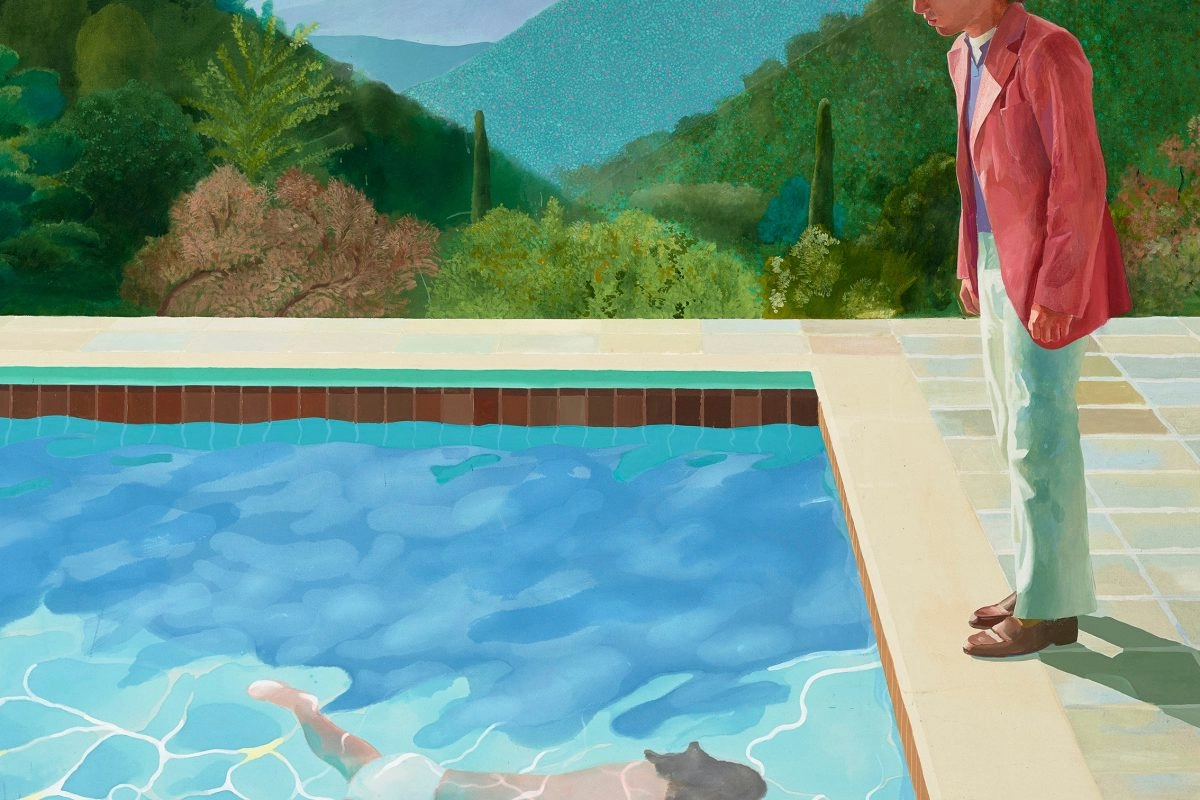
\includegraphics[width=0.7\linewidth]{David_Hockney_Portrait_of_an_Artist.png}
	\end{center}
	\caption{Portrait of an Artist - David Hockney}
	\label{img1}
\end{figure}

\subsection{Ouverture de l'image}

\begin{minted}{python}
image = img.imread('David_Hockney_Portrait_of_an_Artist.png')
plt.imshow(image)
plt.show()

print(image.shape)
\end{minted} 

\begin{exercice}
Après avoir exécuté ce code, expliquer le résultat de la ligne \verb?print(image.shape)?.
\end{exercice}

\begin{solution}~\ \\
Cette ligne affiche la taille de l'image (1200x800), ainsi que le fait qu'il y a 4 caractéristiques par pixel (couleurs RVB et la transparence).
\end{solution}

\subsection{Extraction des couleurs}

Le code suivant permet d'afficher 3 images sur lesquelles seule la composante bleue de l'image originale apparaît.

\begin{minted}{python}
def extraire_couleur(image,id_couleur):
    image_out=image.copy()
    image_out[:,:,0]=0
    image_out[:,:,1]=0
    return image_out

f, axarr = plt.subplots(1,3)
for i in range(3):
    axarr[i].imshow(extraire_couleur(image,i))
plt.show()
\end{minted} 

\begin{exercice}
Proposer une modification de ce code afin qu'il afficher 3 images sur lesquelles apparaissent respectivement les composantes rouge, verte et bleue. Il faudra automatiser cette tâche en utilisant une boucle \verb?for?.
\end{exercice}

\begin{solution}~\\
\vspace{-0.7cm}
\begin{minted}{python}
def extraire_couleur(image,id_couleur):
    image_out=image.copy()
    for i in range(3):
        if i!=id_couleur:
            image_out[:,:,i]=0
    return image_out

f, axarr = plt.subplots(1,3)
for i in range(3):
    axarr[i].imshow(extraire_couleur(image,i))
plt.show()
\end{minted} 
\end{solution}

\subsection{Inversion des couleurs}

Il est possible d'inverser les couleurs d'une image afin d'obtenir son \og négatif \fg. Le principe est de prendre le complément à 1 de chacune des valeurs des couleurs. Ainsi, si une couleur d'un pixel est affectée de la valeur $a$, il faut lui attribuer la valeur $1-a$ pour inverser l'image.

La solution suivante a été envisagée afin de réaliser cette opération, elle consiste à utiliser un tableau rempli de 1 de la taille de l'image et de lui soustraire l'image. Le résultat n'est pourtant pas celui attendu.


\begin{minted}{python}
def inverser_couleur(image):
    image_out=image.copy()
    return np.ones(np.shape(image_out))-image_out

f, axarr = plt.subplots(1,2)
axarr[0].imshow(image)
axarr[1].imshow(inverser_couleur(image))
plt.show()
\end{minted} 

\begin{exercice}
Modifier le code afin de corriger cet erreur, cela permettra d'afficher l'image et son inverse.
\end{exercice}

\begin{solution}~\ \\
Le problème vient du fait que la valeur de l'opacité est de 1 (100\%) pour les deux images. Lors de la soustraction ces deux valeurs s'annulent et l'image est alors transparente (opacité 0). Une solution consiste à rendre transparente l'image à soustraire afin que le résultat ait une opacité de 1 (100\%).
\begin{minted}{python}
def inverser_couleur(image):
    image_out=image.copy()
    image_out[:,:,3]=0
    return np.ones(np.shape(image_out))-image_out

f, axarr = plt.subplots(1,2)
axarr[0].imshow(image)
axarr[1].imshow(inverser_couleur(image))
plt.show()
\end{minted} 
\end{solution}

\subsection{Conversion en niveaux de gris}

Une possibilité de conversion en niveaux de gris s'effectue en faisant la moyenne des trois couleurs et en affectant cette moyenne aux trois couleurs du pixel. Par exemple, si le codage RVBA d'un pixel est $\left[a,b,c,1\right]$, alors, sa conversion en niveaux de gris donnera le résultat suivant $\left[\dfrac{a+b+c}{3},\dfrac{a+b+c}{3},\dfrac{a+b+c}{3},1\right]$.

Le code suivant permet d'afficher ce résultat.

\begin{minted}{python}
def convert_nb_base(image):
    image_out=np.zeros(np.shape(image))
    image_out[:,:,3]=1
    for j in range(3):
        for i in range(3):
            image_out[:,:,j]+=image[:,:,i]/3
    return image_out

plt.imshow(convert_nb_base(image))
plt.show()
\end{minted}

Le résultat n'est pourtant pas optimal car les zones sombres sont trop \og noires \fg. Il a été montré qu'une meilleure solution consiste à utiliser la répartition suivante: $0.2125*rouge+0.7154*vert+0.0721*bleu$, on constate que $0.2125+0.7154+0.0721=1$.


\begin{exercice}
Créer une fonction \verb?convert_nb_evol? qui prend en compte cette répartition et l'utiliser afin de convertir l'image en niveaux de gris. Cette fonction devra être optimisée au maximum grâce à l'utilisation de boucles \verb?for?. Afficher les résultats des deux solutions côte à côte afin de valider le résultat.
\end{exercice}

\begin{solution}~\\
\vspace{-0.7cm}
\begin{minted}{python}
def convert_nb_base(image):
    image_out=np.zeros(np.shape(image))
    image_out[:,:,3]=1
    for j in range(3):
        for i in range(3):
            image_out[:,:,j]+=image[:,:,i]/3
    return image_out

def convert_nb_evol(image):
    image_out=np.zeros(np.shape(image))
    image_out[:,:,3]=1
    coefficients=[0.2125,0.7154,0.0721]
    for j in range(3):
        for i in range(3):
            image_out[:,:,j]+=image[:,:,i]*coefficients[i]
    return image_out

f, axarr = plt.subplots(1,2)
axarr[0].imshow(convert_nb_base(image))
axarr[1].imshow(convert_nb_evol(image))
plt.show()
\end{minted} 
\end{solution}

\subsection{Contraste et luminosité}

La fonction Contraste et luminosité améliore l'apparence d'une image. La luminosité améliore la clarté globale de l'image (par exemple, pour rendre plus claires des couleurs sombres et pour rendre plus pâles des couleurs claires). Le contraste règle la différence entre les couleurs les plus sombres et les couleurs les plus claires.

Pour modifier ces paramètres, il faut appliquer la formule suivante à chaque valeur de couleur de chaque pixel: valeur=contraste*valeur+luminosite, avec 
\verb?contraste? et \verb?luminosite? des valeurs à modifier selon le réglage souhaité.

Attention, il faut veiller à ce que la valeur issue de ce calcul soit toujours comprise entre 0 et 1, sinon il y a aura une erreur à l'exécution. Pour vous aider à cela, vous pouvez aller regarder sur internet la fonction \verb?numpy.clip?.

\begin{exercice}
Créer une fonction \verb?contraste_luminosite? qui permet d'appliquer cet effet à l'image. Afficher l'image initiale et l'image modifiée côte à côte afin de voir l'impact de cet effet.
\end{exercice}
 
\begin{solution}~\\
\vspace{-0.7cm}
\begin{minted}{python}
def contraste_luminosite(image,contraste,luminosite):
    return np.clip(contraste*image+luminosite,0,1)

f, axarr = plt.subplots(1,2)
axarr[0].imshow(image)
axarr[1].imshow(contraste_luminosite(image,2,-0.5))
plt.show()
\end{minted} 
\end{solution}

\subsection{Rotation de l'image de 90°}

Le code suivant permet d'effectuer une rotation de 90° de l'image.

\begin{minted}{python}
def rotation(image):
    return np.rot90(image)

image_rot=image.copy()
f, axarr = plt.subplots(1,4, gridspec_kw={'width_ratios': [3/2, 1,3/2, 1]})
for i in range(4):
    axarr[i].imshow(image_rot)
    axarr[i].title.set_text('Rotation {}°'.format(i*90))
    image_rot=rotation(image_rot)
plt.show()
\end{minted} 

Le principe de la rotation d'une image est présenté sur la figure \ref{img2}.
\begin{figure}[ht!]
	\begin{center}
		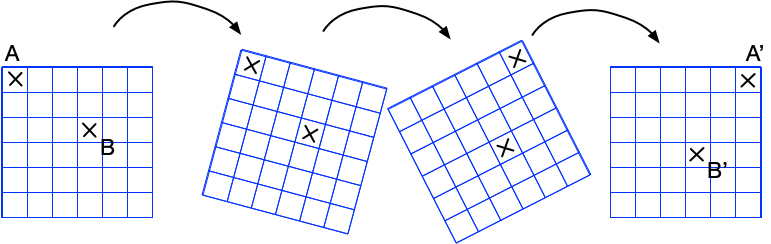
\includegraphics[width=0.7\linewidth]{rotation.png}
	\end{center}
	\caption{Principe de la rotation d'une image pixelisée}
	\label{img2}
\end{figure}

\begin{exercice}
D'après le principe présenté sur la figure \ref{img2}, proposer une solution pour coder vous-même la fonction \verb?rotation? sans l'utilisation de \verb?np.rot90?.
\end{exercice}

\begin{solution}~\\
\vspace{-0.7cm}
\begin{minted}{python}
def rotation(image):
    nb_lig,nb_col,nb_coul=image.shape
    image2=np.zeros((nb_col,nb_lig,nb_coul))
    for i in range(nb_lig):
        for j in range(nb_col):
            for k in range(nb_coul):
                image2[j,i,k]=image[i,nb_col-1-j,k]
    return image2

image_rot=image.copy()
f, axarr = plt.subplots(1,4, gridspec_kw={'width_ratios': [3/2, 1,3/2, 1]})
for i in range(4):
    axarr[i].imshow(image_rot)
    axarr[i].title.set_text('Rotation {}°'.format(i*90))
    image_rot=rotation(image_rot)
plt.show()
\end{minted} 
\end{solution}

\subsection{Réduire la taille d'une image}

Il est parfois utile de réduire la taille d'une image si celle-ci est trop grande pour être manipulée, traitée ou transmise. Le principe consiste à supprimer des pixels.

La fonction suivante permet de le faire.

\begin{minted}{python}
def reduire(image, facteur):
    nb_lig,nb_col,nb_coul=image.shape
    image2=np.zeros((nb_lig//facteur,nb_col//facteur,nb_coul))
    for i in range(nb_lig//facteur):
        for j in range(nb_col//facteur):
            for k in range(nb_coul):
                image2[i,j,k]=image[i*facteur,j*facteur,k]
    return image2

plt.imshow(reduire(image,5))
plt.show()
\end{minted}

\subsection{Augmenter la taille d'une image}

Il peut aussi être intéressant d'augmenter la taille d'une image. Attention, cela n'augmente pas sa qualité car l'information ajoutée est déterminée à partir de l'image de petite taille. L'idée consiste à ajouter des pixels entre les pixels existants et de déterminer les valeurs de leurs couleurs à partir des caractéristiques des pixels proches.

\begin{exercice}
S'inspirer de la fonction \verb?reduire? afin de créer une fonction \verb?agrandir? qui permet d'augmenter la taille d'une image.
\end{exercice}

\begin{solution}~\\
\vspace{-0.7cm}
\begin{minted}{python}
\begin{minted}{python}
def agrandir(image, facteur):
    nb_lig,nb_col,nb_coul=image.shape
    image2=np.zeros((facteur*nb_lig,facteur*nb_col,nb_coul))
    for i in range(facteur*nb_lig):
        for j in range(facteur*nb_col):
            for k in range(nb_coul):
                image2[i,j,k]=image[i//facteur,j//facteur,k]
    return image2

plt.imshow(agrandir(image,2))
plt.show()
\end{minted} 
\end{solution}

\subsection{Détection de contours}

La détection de contours est une technique qui peut être utilisée dans le traitement d'image, afin de faire de la détection d'objets,...

Cela consiste à détecter les gros écarts de contraste entre des pixels à proximité. Pour cela, pour chaque pixel, on regarde la valeur des niveaux de gris de celui décalé de 2 vers la gauche ($p1$), deux en dessous ($p2$), deux vers la droite ($p3$) et deux au-dessus ($p4$), et on calcule la norme $\sqrt{\dfrac{(p1-p3)^2+(p2-p4)^2}{2}}$. Si cette norme est plus grande qu'une valeur \verb?seuil? à définir, on trace un pixel noir sur une nouvelle image blanche. Une fois tous les pixels parcourus les contours apparaissent sur cette image. Il peut alors être intéressant de modifier la valeur \verb?seuil? afin de faire varier la sensibilité aux contours.

\begin{exercice}
Créer la fonction \verb?contour? qui renvoie une image blanche avec les contours en noir dont le fonctionnement est décrit dans le paragraphe précédent.
\end{exercice}

\begin{solution}~\\
\vspace{-0.7cm}
\begin{minted}{python}
def contour(matB):
    normel=[]
    nb_lig,nb_col,nb_coul=matB.shape
    matC=np.zeros((nb_lig,nb_col,nb_coul))
    for i in range(2,nb_lig-2):
        for j in range(2,nb_col-2):
            p1=matB[i-2,j,0]
            p2=matB[i,j-2,0]            
            p3=matB[i+2,j,0]            
            p4=matB[i,j+2,0]
            norme=np.sqrt((p1-p3)**2+(p2-p4)**2)/2
            normel.append(norme)
            seuil=0.15
            if norme < seuil:
                p = 1
            else:
                p = 0               
            for k in range(nb_coul-1):
                matC[i,j,k]=p
            matC[i,j,3]=1
    print(max(normel),min(normel))
    return matC

image=reduire(image,3)
C=convert_nb_evol(image)
D=contour(C)


f, axarr = plt.subplots(1,3)
axarr[0].imshow(image)
axarr[0].title.set_text('Image originale')
axarr[1].imshow(C)
axarr[1].title.set_text('NB')
axarr[2].imshow(D)
axarr[2].title.set_text('Contour')
plt.show()
\end{minted} 
\end{solution}

\end{document}


















